\documentclass[12pt]{article}
\usepackage[small,bf]{caption}
\usepackage{fullpage,graphicx,psfrag,url,ar,rotating,float}
\usepackage{amsmath,amssymb,enumitem,bbm,subcaption,multirow}

\usepackage{pgf,tikz}
\usetikzlibrary{automata,positioning}

\setlength{\captionmargin}{20pt}
\setlist[enumerate]{label=(\roman*)}

\title{\Large{AA274 (Winter 2017-18): Problem Set 2}}
\author{Anqi Fu}

\begin{document}
	\maketitle

\section{Camera Calibration}
\begin{enumerate}
	\item See submitted code. We are given a $7 \times 9$ chessboard grid with each square's side length of $d_{square} = 20.5$ mm. The axes are arranged in traditional fashion with the origin at the bottom left. To generate the world coordinates, we stack the rows of
		\[
			G_X = \left(\begin{array}{cccc}
				0 & d_{square} & \ldots & 8d_{square} \\
				0 & d_{square} & \ldots & 8d_{square} \\
				\vdots & \vdots & \ddots & \vdots \\
				0 & d_{square} & \ldots & 8d_{square}
			\end{array}\right) \quad \mbox{and} \quad
			G_Y = \left(\begin{array}{cccc}
				6d_{square} & 6d_{square} & \ldots & 6d_{square} \\
				5d_{square} & 5d_{square} & \ldots & 5d_{square} \\
				\vdots & \vdots & \ddots & \vdots \\
				0 & 0 & \ldots & 0
			\end{array}\right),
		\]
	producing $(X_k,Y_k) \in \mathbb{Z}_+^{2 \times 63}$ for each of the $k = 1,\ldots,23$ chessboards.
	\item See submitted code. For a given chessboard $i$, form the row vector $\tilde M = (X_k,Y_k,\mathbf{1})^T \in \mathbb{Z}_+^{189}$ by stacking the world coordinates and a 63-length vector of ones. Define
		\[
			L = \left(\begin{array}{ccc}
				\tilde M^T & \mathbf{0}^T & -u_{meas}\tilde M^T \\
				\mathbf{0}^T & \tilde M^T & -v_{meas}\tilde M^T
				\end{array}\right) \in \mathbf{R}^{378 \times 9}
		\]
		and solve $Lx = 0$ by taking the SVD of $L$ and setting $x^*$ equal to the right singular vector associated with the smallest singular value. Then, $x^* = (h_1, h_2, h_3) \in \mathbf{R}^9$ is the stacked columns of our homography matrix $H_k$ for chessboard $k$.
	\item See submitted code. Let the $i$-th column vector of $H_k$ be $h_i = (h_{i1}, h_{i2}, h_{i3})$, and define
		\[
			v_{ij} = \left(\begin{array}{c}
					h_{i1}h_{j1} \\
					h_{i1}h_{j2} + h_{i2}h_{j1} \\
					h_{i2}h_{j2} \\
					h_{i3}h_{j1} + h_{i1}h_{j3} \\
					h_{i3}h_{j2} + h_{i2}h_{j3} \\
					h_{i3}h_{j3}
				\end{array}\right) \quad \mbox{and} \quad
			V_k = \left(\begin{array}{c}
					v_{12}^T \\
					(v_{11} - v_{22})^T
				\end{array}\right)
		\]
		for a particular chessboard $k$. Form $V \in \mathbb{R}^{378 \times 6}$ by stacking the $V_k$ matrices. We can solve $Vb = 0$ by applying the SVD as in the previous part. Given the solution $b^* = (B_{11}, B_{12}, B_{22}, B_{13}, B_{23}, B_{33})$, we can compute
		\begin{align*}
			v_0 &= (B_{12}B_{13} - B_{11}B_{23})/(B_{11}B_{22} - B_{12}^2) \\
			\lambda &= B_{33} - (B_{13}^2 + v_0(B_{12}B_{13} - B_{11}B_{23}))/B_{11} \\
			\alpha &= \sqrt{\lambda/B_{11}} \\
			\beta &= \sqrt{\lambda B_{11}/(B_{11}B_{22} - B_{12}^2)} \\
			\gamma &= -B_{12}\alpha^2\beta/\lambda \\
			u_0 &= \gamma v_0/\beta - B_{13}\alpha^2/\lambda
		\end{align*}
		and form the camera intrinsic matrix
		\[
			A = \left(\begin{array}{ccc}
				\alpha & \gamma & u_0 \\
				0 & \beta & v_0 \\
				0 & 0 & 1
			\end{array}\right)
		\]
	\item See submitted code. Given $A$, we compute for each chessboard
		\[
			q_1 = \lambda A^{-1}h_1, \quad q_2 = \lambda A^{-1}h_2 \quad q_3 = q_1 \times q_2
		\]
		where $h_j$ is column $j$ of $H_k$, and our normalizing factor is $\lambda = 1/\|A^{-1}h_1\|$. Then, we form the matrix $Q = (q_1, q_2, q_3)$ by concatenating the column vectors and take its SVD to get $Q = USV^T$. The desired rotation matrix is $R = UV^T$ with translation $t = \lambda A^{-1}h_3$.
	\item See submitted code. Assuming $f = 1$, the desired transformation comes from the lecture notes:
		\begin{align*}
			\left(\begin{array}{c}
				X_C \\
				Y_C \\
				Z_C
			\end{array}\right) = \left(\begin{array}{cc} R & t\end{array}\right)\left(\begin{array}{c}
				X \\
				Y \\
				Z \\
				\mathbf{1}
			\end{array}\right) \quad &\Rightarrow \quad \left(\begin{array}{c}
											x \\
											y
										\end{array}\right) = \left(\begin{array}{c}
											X_C/Z_C \\
											Y_C/Z_C
										\end{array}\right) \\
			\left(\begin{array}{c}
			x_h \\
			y_h \\
			z_h
			\end{array}\right) = A\left(\begin{array}{cc} R & t\end{array}\right)\left(\begin{array}{c}
			X \\
			Y \\
			Z \\
			\mathbf{1}
			\end{array}\right) \quad &\Rightarrow \quad \left(\begin{array}{c}
			u \\
			v
			\end{array}\right) = \left(\begin{array}{c}
			x_h/z_h \\
			y_h/z_h
			\end{array}\right)
		\end{align*}
	\item See submitted code. Given $k = (0.15, 0.01)$, we can solve for
		\begin{align*}
			\breve x &= x + x(k_1(x^2 + y^2) + k_2(x^2 + y^2)^2) \\
			\breve y &= y + y(k_1(x^2 + y^2) + k_2(x^2 + y^2)^2) \\
			\breve u &= u_0 + \alpha \breve x + \gamma \breve y \\
			\breve v &= v_0 + \beta \breve y
		\end{align*}
\end{enumerate}

\section{Line Fitting}
\begin{enumerate}
	\item See submitted code.
	\item Using the suggested algorithm, we extracted the following lines for each data set.
	\begin{figure}[H]
		\centering
		\title{\bf Range Data $(x_r, y_r, n_{pts}) = (5,5,180)$ \\ \vspace{2.5mm}
			\verb|LINE_POINT_DIST_THRESHOLD = 0.05| \\
			\verb|MIN_POINTS_PER_SEGMENT = 0.065| \\
			\verb|MIN_SEG_LENGTH = 2| \\
			\verb|MAX_P2P_DIST = 0.8|}
		\\ \vspace{5mm}
		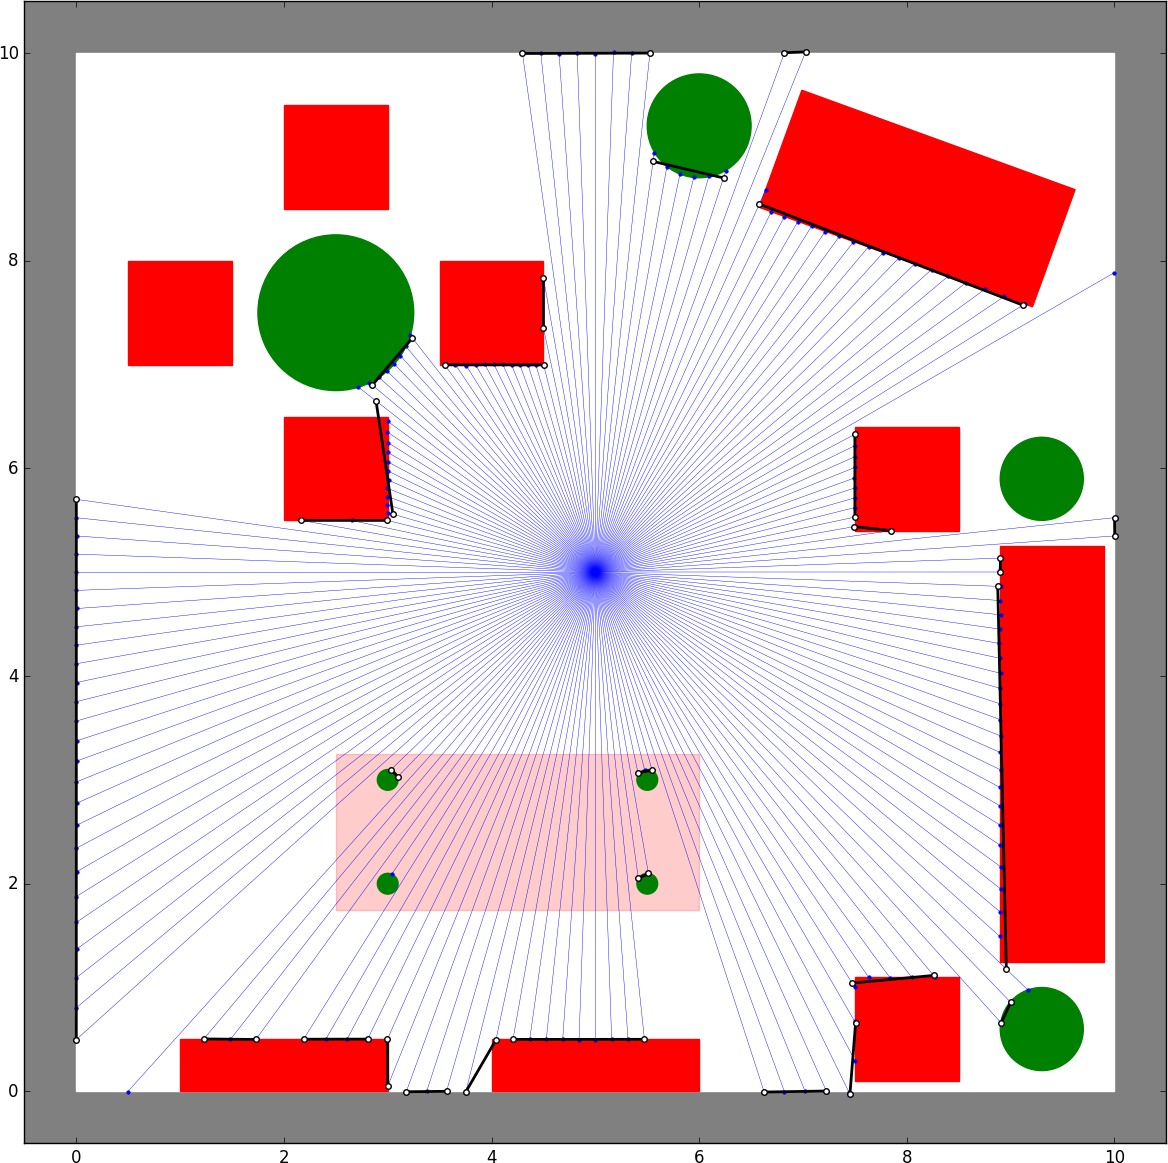
\includegraphics[width=0.8\textwidth]{../Figures/hw2_2_ii_55180.png}
	\end{figure}
	\begin{figure}[H]
		\centering
		\title{\bf Range Data $(x_r, y_r, n_{pts}) = (4,9,360)$ \\ \vspace{2.5mm}
			\verb|LINE_POINT_DIST_THRESHOLD = 0.05| \\
			\verb|MIN_POINTS_PER_SEGMENT = 0.025| \\
			\verb|MIN_SEG_LENGTH = 3| \\
			\verb|MAX_P2P_DIST = 0.54|}
		\\ \vspace{5mm}
		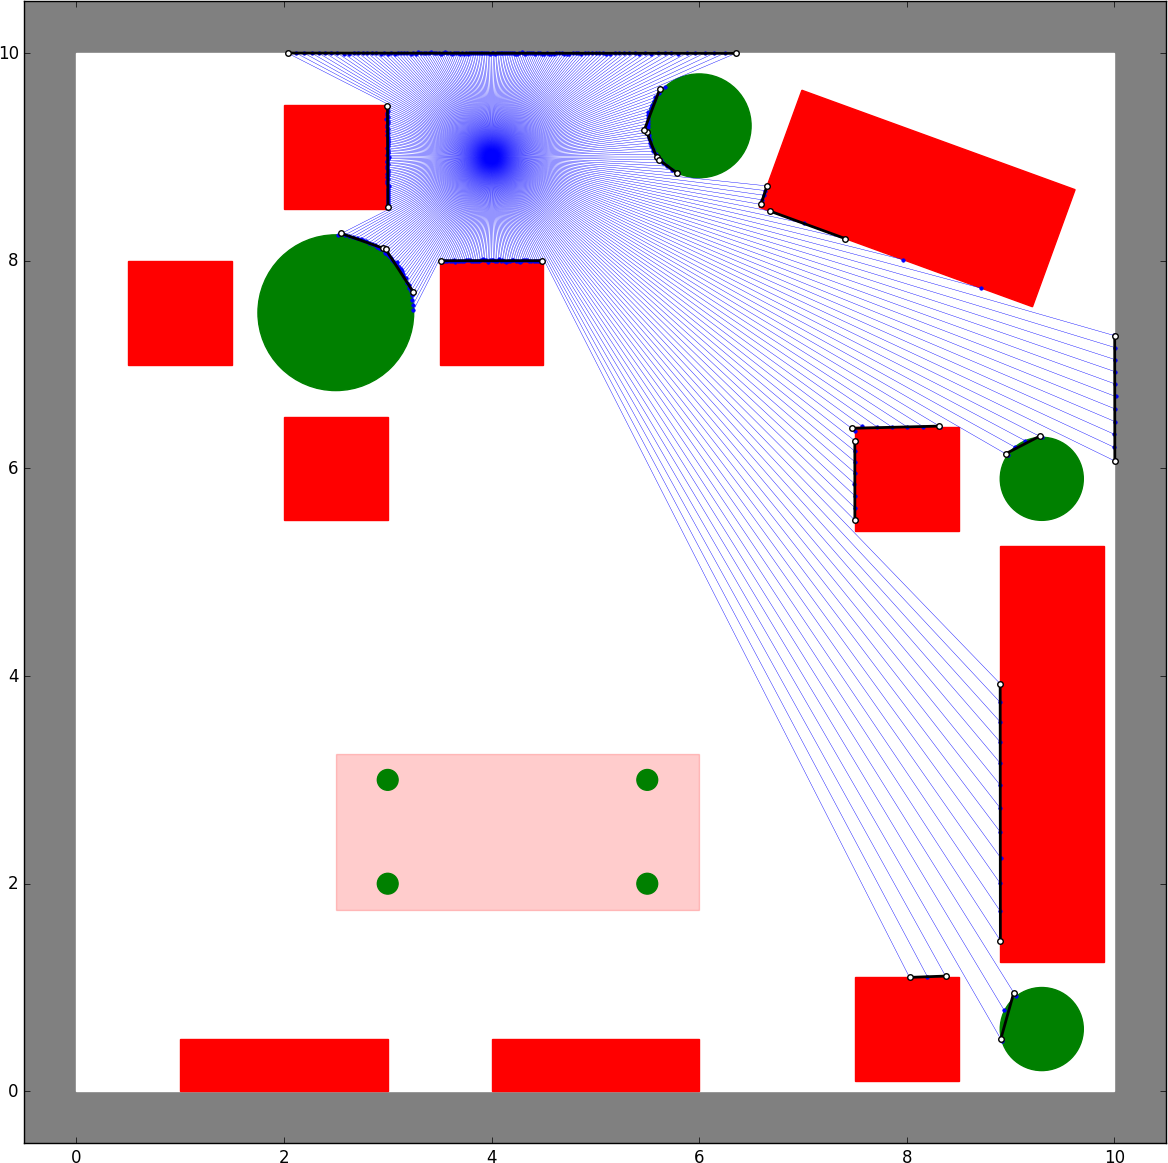
\includegraphics[width=0.8\textwidth]{../Figures/hw2_2_ii_49360.png}
	\end{figure}
	\begin{figure}[H]
		\centering
		\title{\bf Range Data $(x_r, y_r, n_{pts}) = (7,2,90)$ \\ \vspace{2.5mm}
			\verb|LINE_POINT_DIST_THRESHOLD = 0.05| \\
			\verb|MIN_POINTS_PER_SEGMENT = 0.165| \\
			\verb|MIN_SEG_LENGTH = 2| \\
			\verb|MAX_P2P_DIST = 0.42|}
		\\ \vspace{5mm}
		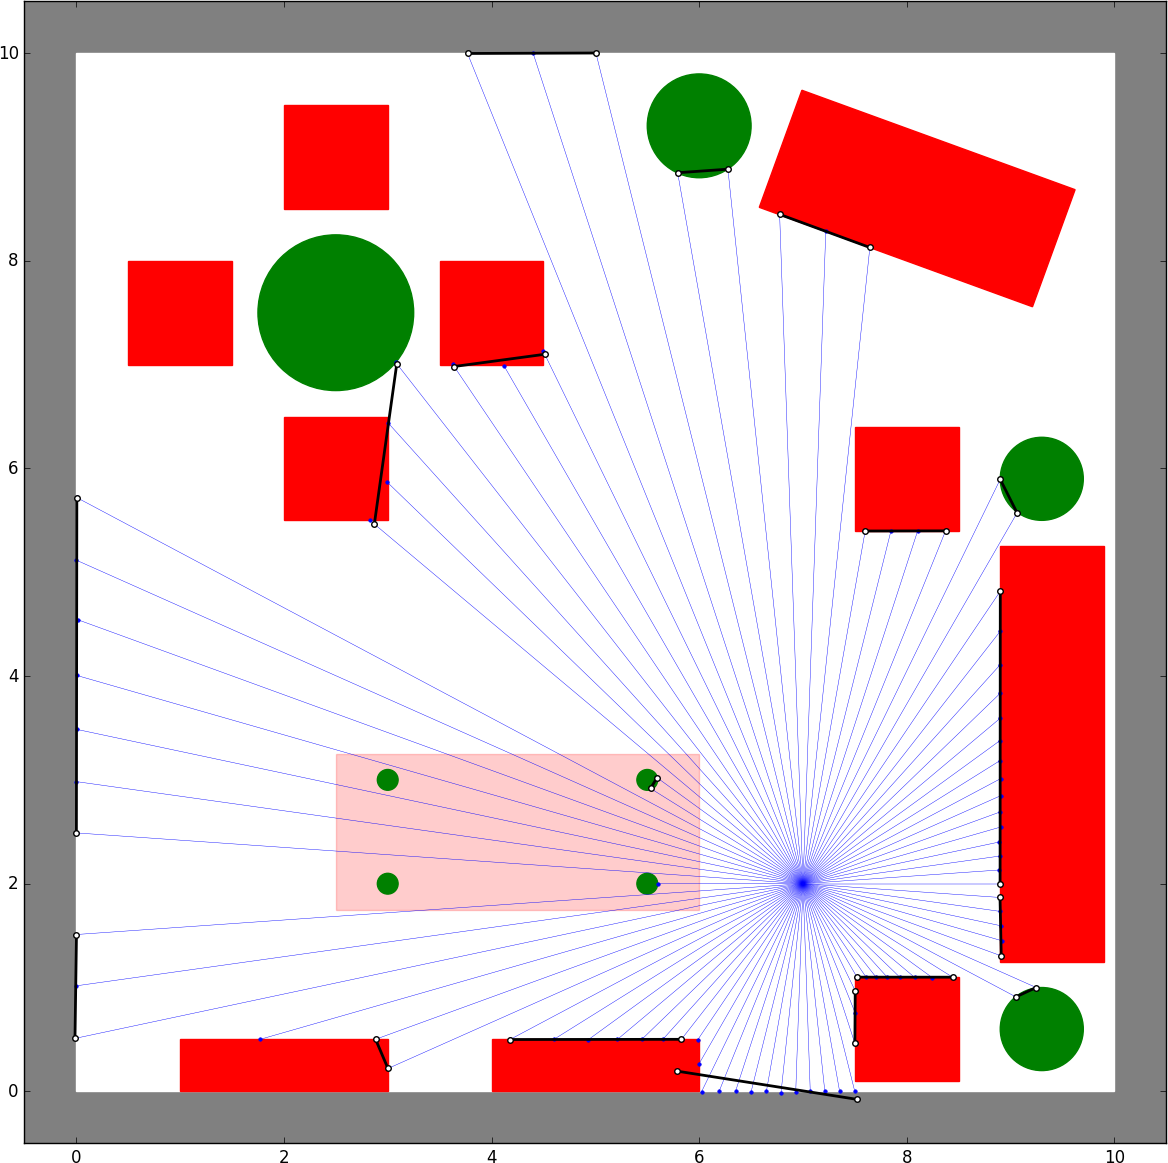
\includegraphics[width=0.8\textwidth]{../Figures/hw2_2_ii_7290.png}
	\end{figure}
\end{enumerate}

\section{Tensorflow and HOG + SVM Pedestrian Detection}
\begin{enumerate}
	\item Let $p, q \in \mathbb{R}^2$ be two points on the parallel hyperplanes, i.e. $w \cdot p - b = 1$ and $w \cdot q - b = -1$. The perpendicular distance between the planes is the projection of the vector $(p - q)$ onto the unit normal to the plane, $\frac{w}{\|w\|}$, which is simply
	\[
		(p - q) \cdot \frac{w}{\|w\|} = \frac{w \cdot p - w \cdot q}{\|w\|} = \frac{(b+1) - (b-1)}{\|w\|} = \frac{2}{\|w\|}
	\]
	\item TensorFlow's workflow was created for modeling and executing distributed computations. The computation graph allows the user to see which mathematical operations will occur in parallel, making it easier to design and debug algorithms. Moreover, the actual data analysis is separated into another step to facilitate execution across multiple, distributed machines. Problems with the algorithm can thus be isolated from problems with the devices that carry out the computation, such as a breakdown in communication. This workflow differs from numpy, which immediately executes operations in the order they are entered. TensorFlow's paradigm makes sense for machine learning, because in this space, algorithms are complex and datasets are generally very large, requiring significant runtime on multiple machines. To avoid wasting resources, users will first test their computation graph locally before starting a cluster and feeding it the input data.
	\item See submitted code.
	\item With a learning rate of $\gamma = 0.1$ and $\lambda = 0.4$, I achieved a misclassification rate of 0.214 on the test dataset. This is rather high because the classes cannot be separated by a single hyperplane. The red class has curved boundaries on both top and bottom with the blue class. Thus, no matter where we draw the hyperplane, a large proportion of the classes will be misclassified. This model has placed it along the top boundary, so that all the blue points below it are labeled as red.
	\begin{figure}[H]
		\centering
		\title{\bf Misclassified Data with Original Features \\
			($\gamma = 0.1, \; \lambda = 0.4$)}
		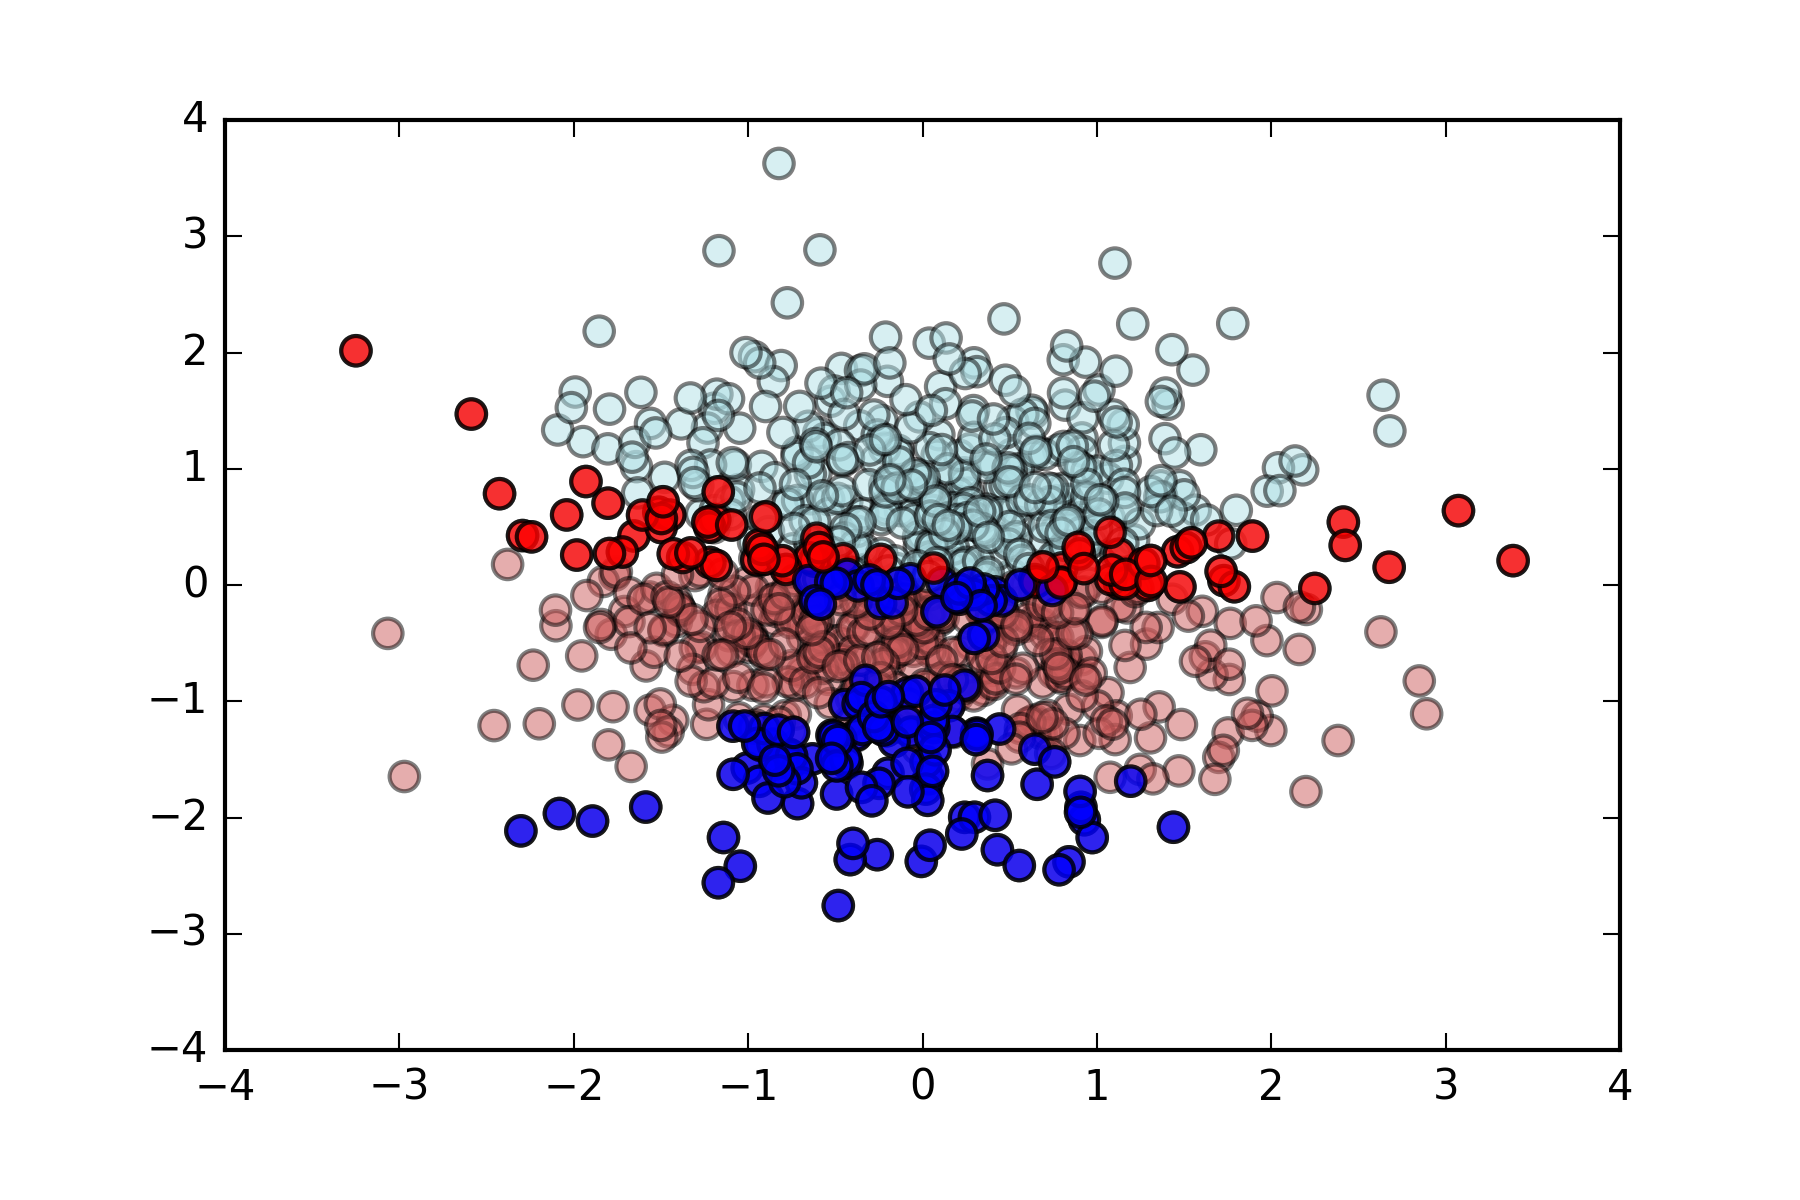
\includegraphics[width=0.8\textwidth]{../Figures/hw2_3_iv.png}
	\end{figure}
	\item See submitted code.
	\item I selected the features $(x_1, x_2, x_1^2, x_2^2, x_1x_2)$ because the boundaries between the two classes look like parabolas, so I expected there to be a quadratic dependency in the data. With a learning rate of $\gamma = 0.1$ and $\lambda = 1.1$, I achieved a misclassification rate of 0.120 on the test dataset.
	\begin{figure}[H]
		\centering
		\title{\bf Misclassified Data with Custom Features \\
			($\gamma = 0.1, \; \lambda = 1.1$)}
		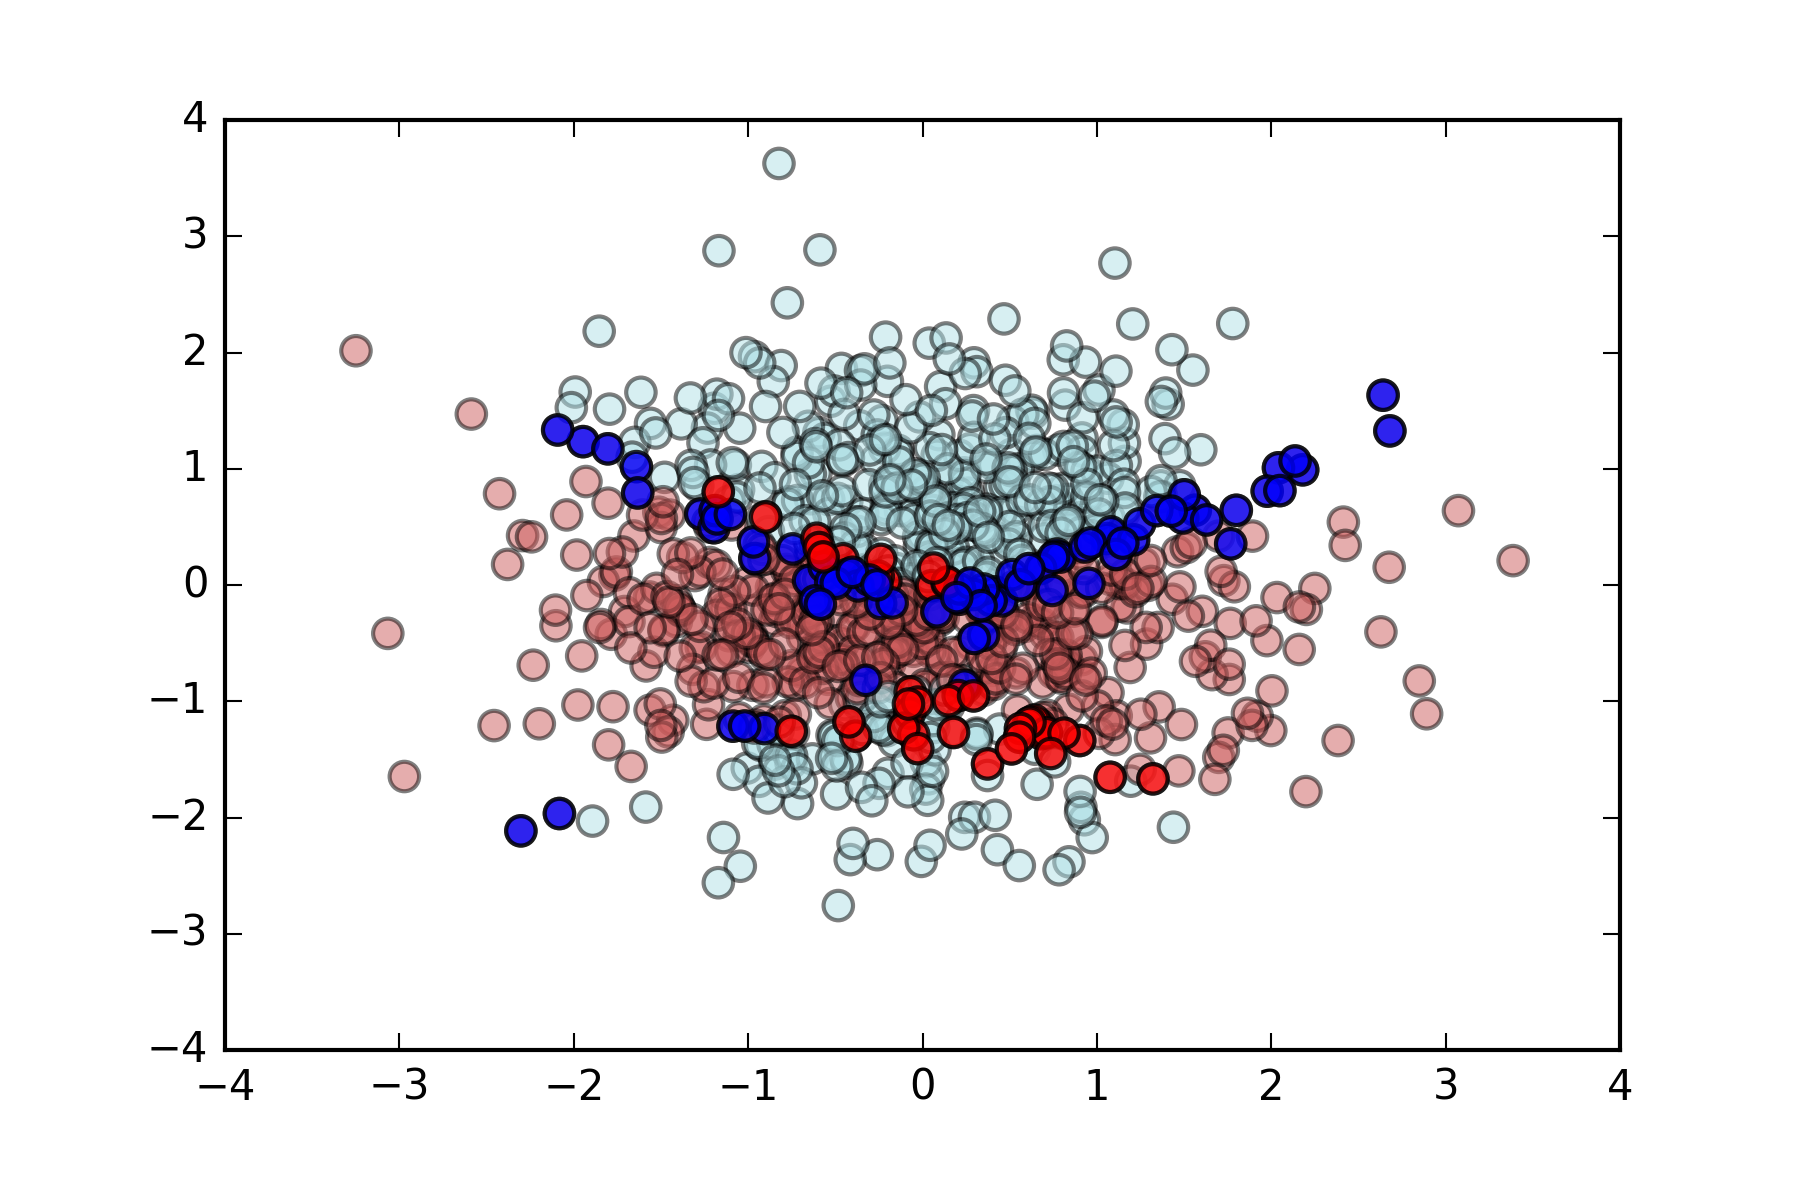
\includegraphics[width=0.8\textwidth]{../Figures/hw2_3_vi.png}
	\end{figure}
	\item See submitted code.
	\item With a learning rate of $\gamma = 0.075$ and $\lambda = 0.825$, I achieved a misclassification rate of 0.130 on the test dataset.
\end{enumerate}

\section{Classification and Sliding Window Detection}
\begin{enumerate}
	\item By examining \verb|bottleneck_input/BottleneckInputPlaceholder| in the \verb|final_training_ops| node, we see that each bottleneck image summary has dimension $1 \times 2048$. There are 3 bias inputs and $2048 \times 3$ weights for a total of 6147 parameters. I achieved a misclassification rate of 0.10 ($15 / 150$) on the test dataset.
	\item See submitted code.
	\item See submitted code. Below, I display the results on \verb|catswithdogs/007417.jpg| with window padding on each side of about 15\% the total height/width.
	\begin{figure}[H]
		\centering
		\title{\bf Brute Force Classification \\
			Padding: 40 px (height), 75 px (width)}
		\\ \vspace{5mm}
		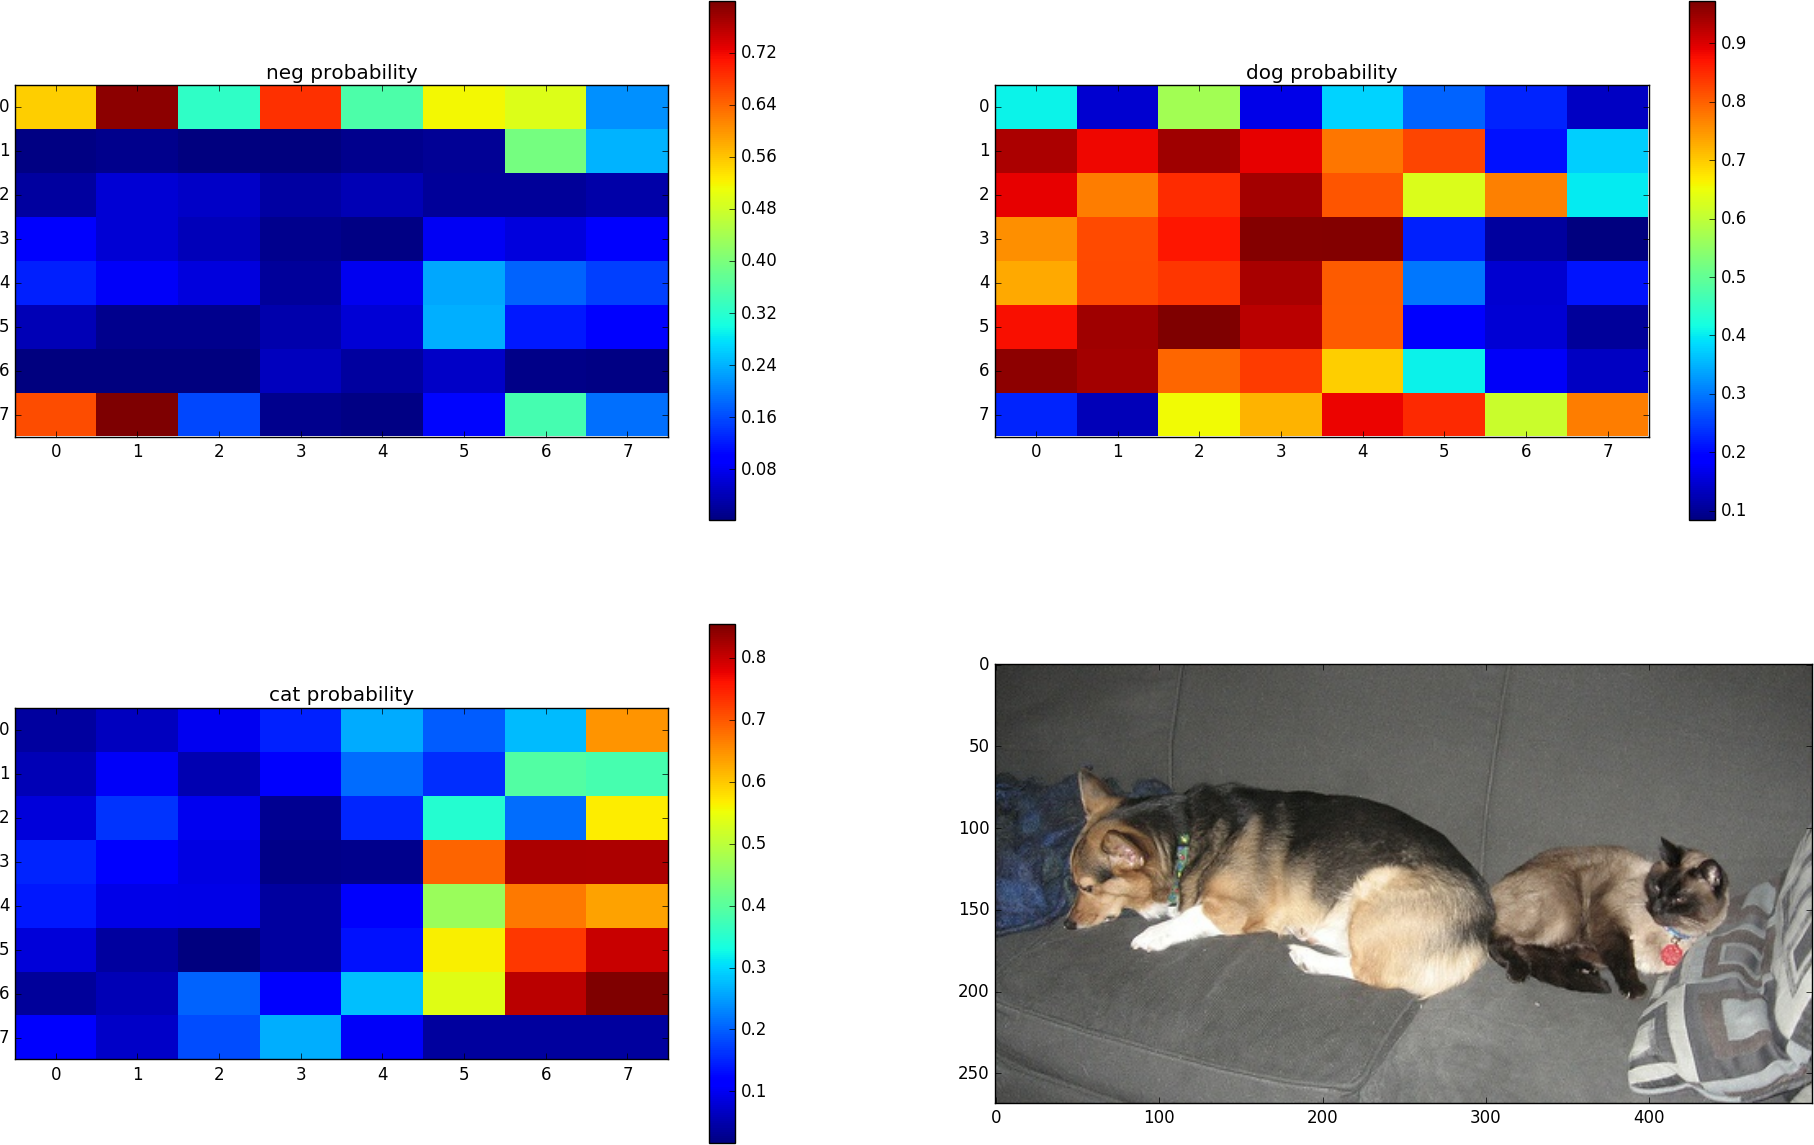
\includegraphics[width=0.9\textwidth]{../Figures/hw2_4_iii_catswithdogs_007417.png}
	\end{figure}
	\item See submitted code.
	\begin{figure}[H]
		\centering
		\title{\bf Convolutional $K \times K$ Classification}
		\\ \vspace{5mm}
		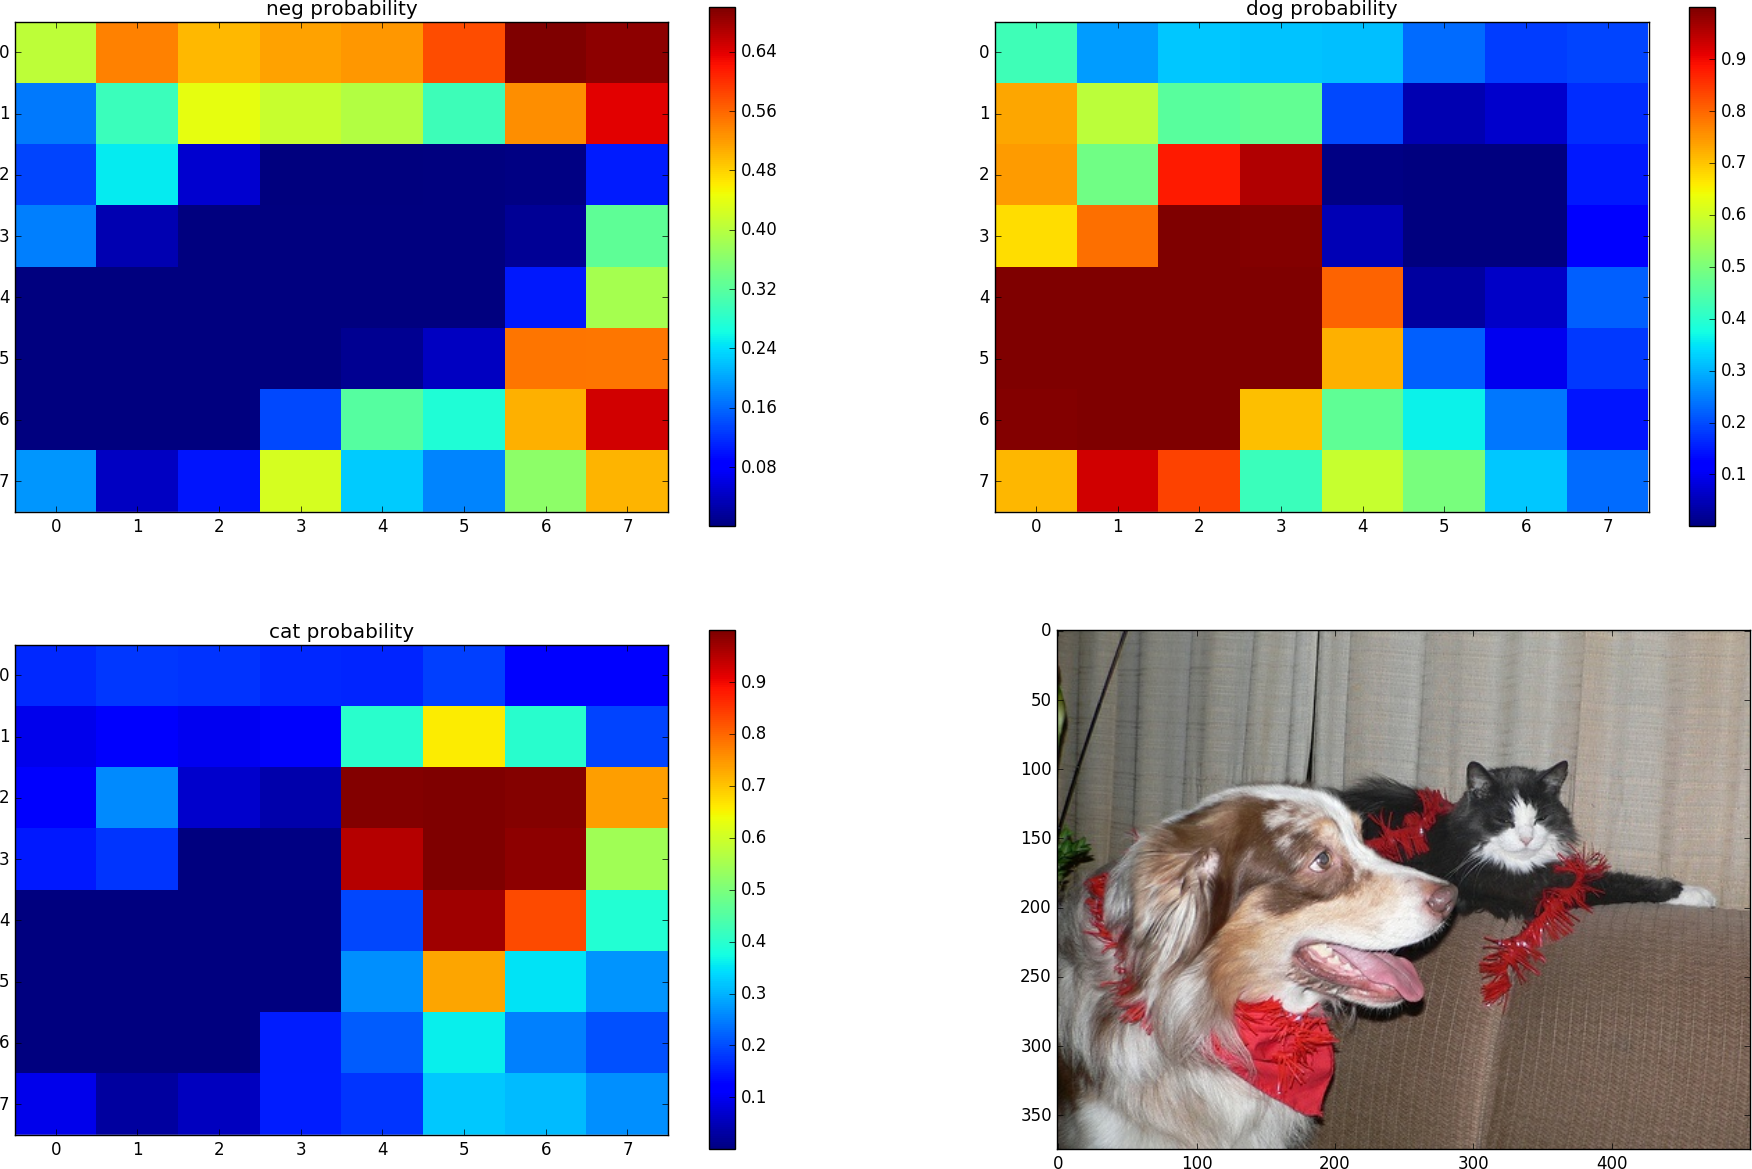
\includegraphics[width=0.9\textwidth]{../Figures/hw2_4_iv_catswithdogs_006026.png}
	\end{figure}
	\item The output of the final convolutional layer, \verb|mixed_10/join:0|, feeds into the node \verb|pool_3/(pool_3)|, which performs the AvgPool operation across the $8 \times 8$ windows. Thus, the feature vector for the image as a whole is the average of the feature vectors for each image region.
	\item See submitted code. Given the raw gradient matrix $w \in \mathbb{R}^{m \times n \times p}$, we calculate the class saliency map to be $M \in \mathbb{R}^{m \times n}$ with entries $M_{ij} = \max_c |w_{ijc}|$, i.e. the maximum magnitude of $w$ across all color channels.
	\item I compute and plot the saliency map for test image \verb|000516.png|, which was correctly classified as a cat. In contrast, test image \verb|004831.png| depicts neither a cat nor a dog, but was misclassified as a cat with class probabilities $(P_{neg}, P_{dog}, P_{cat}) = (0.23824486, 0.2742611, 0.48749402)$. From the saliency, it is clear that the classifier detected the baby as a cat, possibly due to the angle of the photo and light saturation along the arm.
	\begin{figure}[H]
		\centering
		\title{\bf Correctly Classified Image (Cat)}
		\\ \vspace{2.5mm}
		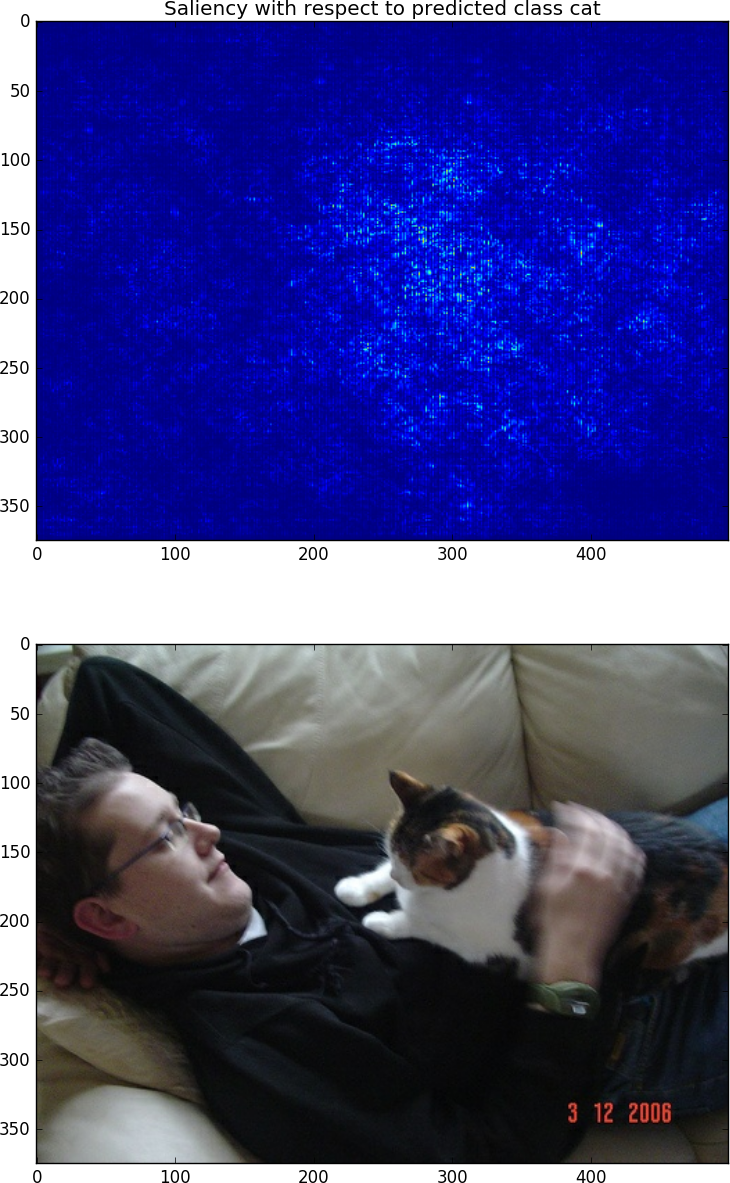
\includegraphics[height=0.8\textheight]{../Figures/hw2_4_vii_test_cat_000516.png}
	\end{figure}
	\begin{figure}[H]
		\centering
		\title{\bf Misclassified Image (Neg)}
		\\ \vspace{2.5mm}
		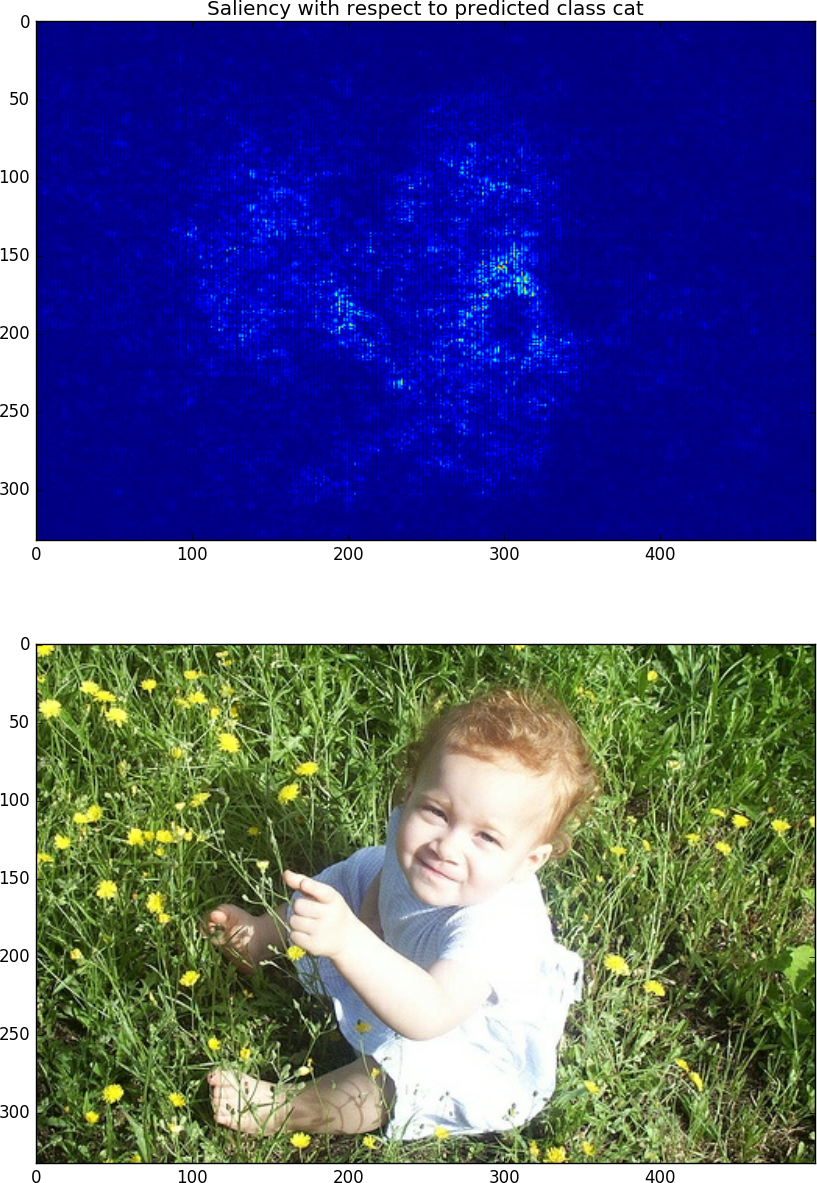
\includegraphics[height=0.8\textheight]{../Figures/hw2_4_vii_test_neg_004831.png}
	\end{figure}
\end{enumerate}

\section{Stop Sign Detection and FSM in ROS}
\begin{enumerate}
	\item \verb|supervisor.py| publishes the current desired pose, which is a message of type \verb|Pose2D| that contains the goal position $(x_g,y_g,\theta_g)$.
	\item See submitted code.
	\item See submitted code.
	\item See submitted code. From Figure 13, we can solve for
	\begin{equation}\label{eqn:5_4_norm}
		\frac{\tilde x - \tilde x_0}{f_x} = \frac{X_C}{Z_C} \quad \mbox{and} \quad \frac{\tilde y - \tilde y_0}{f_y} = \frac{Y_C}{Z_C}
	\end{equation}
	Then, $Z_C$ is determined by the unit vector constraint
	\begin{align*}
		1 &= X_C^2 + Y_C^2 + Z_C^2 \\ 
		\frac{1}{Z_C^2} &= \left(\frac{X_C}{Z_C}\right)^2 + \left(\frac{Y_C}{Z_C}\right)^2 + 1 \\
		Z_C &= \left[\left(\frac{\tilde x - \tilde x_0}{f_x}\right)^2 + \left(\frac{\tilde y - \tilde y_0}{f_y}\right)^2 + 1\right]^{-\frac{1}{2}}
	\end{align*}
	which we can plug back into (\ref{eqn:5_4_norm}) to get $X_C$ and $Y_C$.
	\item TODO: Define input/output, label, and behavior of each state.
	\begin{center}
	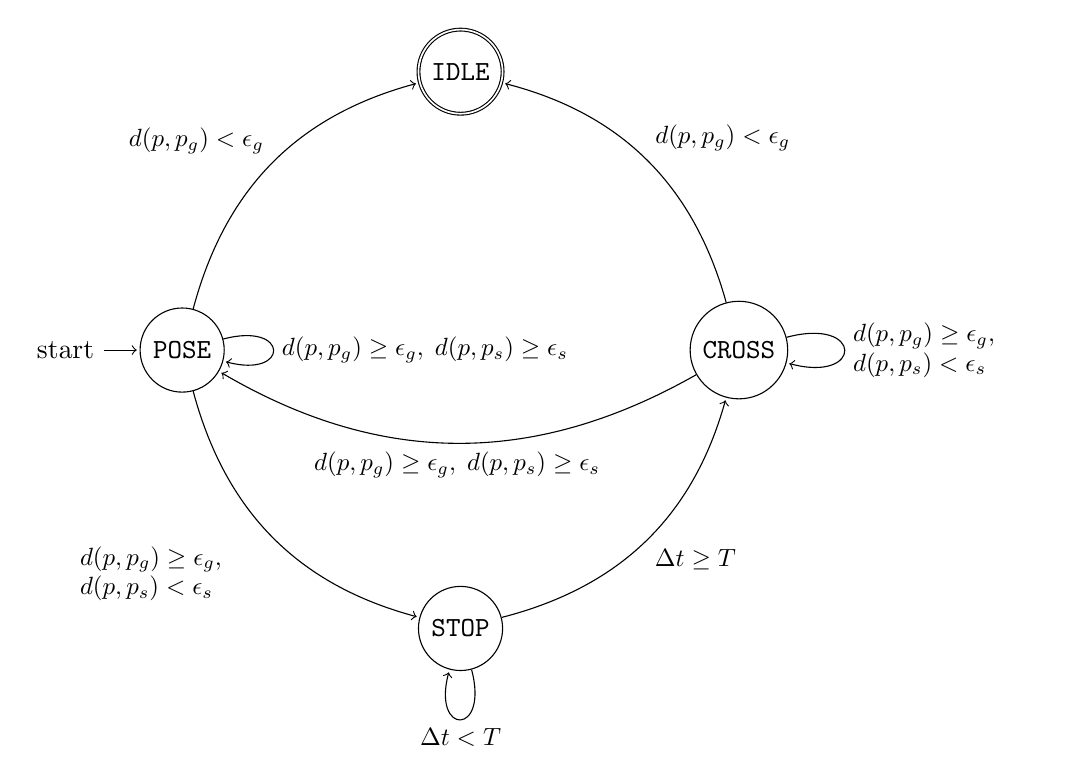
\begin{tikzpicture}[shorten >= 1pt, node distance=5cm, on grid, auto]
		\node[state, initial] (s_0)             {\verb|POSE|};
		\node[state, accepting] (s_1) [above right=of s_0] {\verb|IDLE|};
		\node[state] (s_2) [below right=of s_0] {\verb|STOP|};
		\node[state] (s_3) [below right=of s_1] {\verb|CROSS|};
		
		\begin{scope}[every node/.style={scale=0.9}]
		\path[->]
		(s_0) edge[bend left]  node {$d(p,p_g) < \epsilon_g$} (s_1)
		      edge[loop right] node {$d(p,p_g) \geq \epsilon_g, \; d(p,p_s) \geq \epsilon_s$} (s_0)
		      edge[bend right] node[text width=2.6cm, swap] {$d(p,p_g) \geq \epsilon_g$, \\ $d(p,p_s) < \epsilon_s$} (s_2)
		(s_2) edge[bend right] node[swap] {$\Delta t \geq T$} (s_3)
		      edge[loop below] node {$\Delta t < T$} (s_2)
		(s_3) edge[bend right] node[swap] {$d(p,p_g) < \epsilon_g$} (s_1)
		      edge[loop right] node[text width=2.6cm] {$d(p,p_g) \geq \epsilon_g$, \\ $d(p,p_s) < \epsilon_s$} (s_3)
		      edge[bend left]  node {$d(p,p_g) \geq \epsilon_g, \; d(p,p_s) \geq \epsilon_s$} (s_0);
		\end{scope}
	\end{tikzpicture}
	\end{center}
	\item See submitted code.
	\item TODO
\end{enumerate}
\end{document}